\documentclass[french, 12pt]{article}%

\usepackage[utf8]{inputenc}  
\usepackage[francais]{babel}
\usepackage{appendix}
\usepackage{pdfpages} 
\usepackage{eurosym}
\usepackage{enumitem}
%\usepackage[T1]{fontenc}

%%%%%%%%%%%%%%%%%%%%%%%%%%%%%%%%%%%%%%%%%%%%%%%%%%%%%%%%%
\newcommand{\itemE}{\item[$\bullet$]}
\newcommand{\titreSeq}{Dump device}
\newcommand{\lycee}{Lycée Brocéliande}
\newcommand{\classSeq}{CIEL }
\newcommand{\matiereSeq}{IR}      
\newcommand{\numSeq}{06}
\newcommand{\numAct}{03}
\newcommand{\objSeance}{Le pirate a-t-il capitulé?}

\newcommand{\moySeq}{\begin{itemize}	
\itemE Esp32
\itemE IDE de programmation ESP32
\itemE Machine windows
\itemE Virtual Machine
\end{itemize}}

\newcommand{\compSeq}{\begin{itemize}
\item  
\end{itemize}}
%%%%%%%%%%%%%%%%%%%%%%%%%%%%%%%%%%%%%%%%%%%%%%%%%%%%%%%%%%

%%%%%%%%%%%%%%%%%%%%%%%%%%%%%%%%%%%%%%%%%%%%%%%%%%%%%%%%
%%%%Algo
\usepackage[linesnumbered, french]{algorithm2e}
\SetKwFor{For}{Pour}{faire}{fin}
\SetKwFor{While}{Tant que}{faire}{fin}%
\SetKw{KwTo}{à}
\SetKw{KwPas}{par pas de}
\SetKw{KwRet}{Retourne}
\SetKwProg{Fn}{Fonction }{ arguments }{fin}
\SetKwRepeat{Repeat}{Répéter}{jusqu'à}%
\SetKwIF{If}{ElseIf}{Else}{Si}{alors}{Sinon si}{Sinon}{Fin}

\usepackage{listings} %%%%Présenration code source
\lstset{language=C++,
    %numbers=left,
   %stepnumber=1,
    showstringspaces=false,
    tabsize=1,
    breaklines=true,
    breakatwhitespace=false,
    basicstyle=\footnotesize,
    keywordstyle=\color{blue}\footnotesize,
    stringstyle=\color{red}\footnotesize,
    commentstyle=\color{magenta}\footnotesize,
    morecomment=[l][\color{magenta}]{\#}
    }
\lstdefinestyle{commande}{
  basicstyle=\ttfamily\footnotesize,
  keywordstyle=\color{blue},
  commentstyle=\color{gray},
  %numbers=left,
  %numberstyle=\tiny\color{gray},
  numbersep=5pt,
  breaklines=true,
  frame=single,
  backgroundcolor=\color{lightgray!10}
  %captionpos=b,
  %caption=\lstname  
}
%\usepackage[T1]{fontenc}


% Margins
\topmargin=-0.45in
\evensidemargin=0in
\oddsidemargin=0in
\textwidth=6.5in
\textheight=9.0in
\headsep=0.25in 


\linespread{1.1} 
\usepackage{amsmath}%
\usepackage{amsfonts}%
\usepackage{amssymb}%
\usepackage{graphicx}
\usepackage{lastpage}
\usepackage{enumitem}

%\usepackage[T1]{fontenc}    
\usepackage{multirow}
\usepackage{lscape}
\usepackage[colorlinks = true,
            linkcolor = blue,
            urlcolor  = blue,
            citecolor = blue,
            anchorcolor = blue]{hyperref}
\usepackage{array}
\usepackage{mwe}
%-------------------------------------------
\newtheorem{theorem}{Theorem}
\newtheorem{summary}[theorem]{Summary}
\newenvironment{proof}[1][Proof]{\textbf{#1.} }{\ \rule{0.5em}{0.5em}}



\usepackage{xcolor}

\usepackage{colortbl}
\setlength{\doublerulesep}{\arrayrulewidth}
%-------------------------------------------
%%%%%%%%%%%%%%%%%%%%%%%%%%%%%%%%%%%%%%%%%%%%%
\usepackage[framemethod=tikz]{mdframed}
\usepackage{tikz, xcolor, lipsum}
\makeatletter
\mdfsetup{skipabove=\topskip,skipbelow=\topskip}

\tikzset{titre_bleu_snir/.style =
	{draw=vert_capet, line width=1.5pt, fill=white,
	rectangle, rounded corners, right,minimum height=2em}}
\newcommand{\titreencadre}{Titre}
\makeatletter
\mdfdefinestyle{encadrestyle}{%
	linewidth=1.5pt,roundcorner=5pt,linecolor=vert_capet,
	apptotikzsetting={\tikzset{mdfbackground/.append style ={%
		fill=white}}},
	frametitlefont=\bfseries,
	singleextra={%
		\node[titre_bleu_snir,xshift=2em] at (P-|O) %
			{~\mdf@frametitlefont{\titreencadre}\hbox{~}};},
	firstextra={%
		\node[titre_bleu_snir,xshift=2em] at (P-|O) %
		{~\mdf@frametitlefont{\titreencadre}\hbox{~}};},
	}
\mdfdefinestyle{encadresanstitrestyle}{%
	linewidth=1.5pt,roundcorner=5pt,linecolor=vert_capet
	apptotikzsetting={\tikzset{mdfbackground/.append style ={%
		fill=yellow!20}}},
	}

\newenvironment{encadre}[1]{\renewcommand{\titreencadre}{#1}
	\begin{mdframed}[style=encadrestyle]
	\vspace{0.5\baselineskip}
	}{%
	\end{mdframed}}

\newenvironment{encadresanstitre}{
	\begin{mdframed}[style=encadresanstitrestyle]
	}{%
	\end{mdframed}}
\makeatother
\usepackage{colortbl}
\definecolor{vert_capet}{RGB}{191,255,191}	
\definecolor{bleu_snir}{RGB}{191,255,191} %%{101,191,179}	
\setlength{\doublerulesep}{\arrayrulewidth}
%-------------------------------------------
\usepackage{comment}
%%%%%%%%%%%%%%%%%%%%%%%%%%%%%%%
\newif\ifPROF

%\def\PourProf{0}
\ifdefined\PourProf
  \PROFtrue
  \newenvironment{corr}{\begingroup \color{red}}{\normalcolor \endgroup}
\else
  \PROFfalse
  \newenvironment{corr}{\begingroup \color{white}}{\normalcolor \endgroup}
\fi
%\PROFtrue

%%%%%%%%%%%%%%%%%%%%%%%%%%%%%%%%%%%%




%%%Note et pied de page
\usepackage{fancybox}
\usepackage{fancyhdr}
\usepackage[a4paper,margin=2.5cm,bottom=2cm,headheight=2cm]{geometry}
\pagestyle{fancy}
\fancyhead[R]{
\includegraphics[scale=0.3]{logo_CIEL.png}}
\fancyhead[C]{Prénom}
\fancyhead[L]{Nom}
\fancyfoot[C]{Page \thepage/\pageref{LastPage}}
\fancyfoot[L]{\classSeq ~\matiereSeq}
\fancyfoot[R]{Seq \numSeq  ~ Act \numAct}
\renewcommand{\headrulewidth}{1pt}
%%%Note et pied de page 



\begin{document}

\title{\titreSeq\\
 
\includegraphics[scale=0.5]{logo_CIEL.png}\\
}
\author{\lycee}
\date{}%\today}
%\maketitle

\noindent\begin{tabular}{!{\vrule width 1.5pt}m{0.7\linewidth}!{\vrule width 1.5pt}m{0.2\linewidth}!{\vrule width 1.5pt}}
\hline\hline
\cellcolor{bleu_snir}
\begin{center}
	\Large\textbf{\titreSeq}  
\end{center}
  & 

\begin{minipage}{1.0\linewidth}
  \vspace*{0.1cm} 
\centering
\includegraphics[scale=0.2]{logo_lycee.jpg}

{\tiny\today}
  \vspace*{0.1cm} 
\end{minipage}\\ \hline\hline

\multicolumn{2}{!{\vrule width 1.5pt}l!{\vrule width 1.5pt}}{
\begin{minipage}{14cm}
\vspace*{0.1cm} 
\textbf{Objectif} : \objSeance
\vspace*{0.1cm} 
\end{minipage}} \\ \hline\hline

\multicolumn{2}{!{\vrule width 1.5pt}l!{\vrule width 1.5pt}}{
\begin{minipage}{14cm}
\vspace*{0.1cm} 
\textbf{Moyens} : 
\moySeq
\vspace*{0.1cm} 
\end{minipage}} \\ \hline\hline
%
%\multicolumn{2}{!{\vrule width 1.5pt}l!{\vrule width 1.5pt}}{
%\begin{minipage}{14cm}
%\vspace*{0.1cm}
%\tiny
%Compétences attendues :
%\compSeq
%\vspace*{0.1cm}
%\end{minipage}}
%\normalsize \\ \hline\hline
\end{tabular}

%%%%%%%%%%%%%%%%%%%%%%%%%%%%%%%%%%%%%%%%%%%%%%%%%%%%%%%%%%%%%%%%%%%%%%%%%%%%%%%%
\vspace{0.25cm}

%%%%%%%%%%%%%%%%%%%%%%%%%%%%%%%%%%%%%%%%%%%%%%%%%%%%%%%%%%%%%%%%%%%%%%%%%%%%%%%%%%%%%%%%%%%%%%%
%%%%%%%%%%%%%%%%%%%%%%%%%%%%%%  DEBUT %%%%%%%%%%%%%%%%%%%%%%%%%%%%%%%%%%%%%%%%%%%%%%%%%%%%%%%%%
%%%%%%%%%%%%%%%%%%%%%%%%%%%%%%%%%%%%%%%%%%%%%%%%%%%%%%%%%%%%%%%%%%%%%%%%%%%%%%%%%%%%%%%%%%%%%%%

\section{Contexte}

Précédemment, dans la salle de concert ZenithCiel, vous avez mis en avant un vulnérabilité : 
\begin{itemize}
\itemE Clef Wifi trop faible
\itemE Des personnes mal intentionnée pouvaient usurper l'identité d'un capteur et donc envoyer des informations erronées au serveur
\end{itemize}

Vous avez ensuite proposé une solution basée sur des certificats pour sécuriser les échanges (Authentification et confidentialité).

Pour rappel, l'infrastructure est la suivante : 

\begin{center}
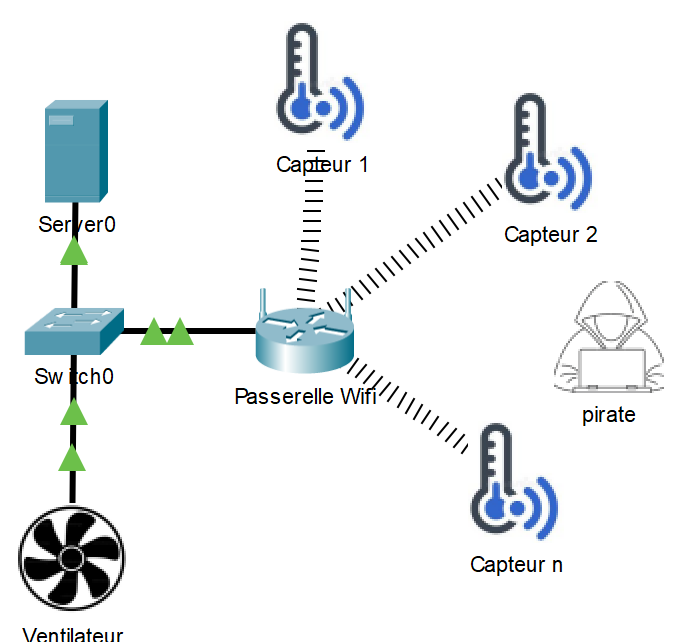
\includegraphics[scale=0.4]{./ressource/topologIeWifiEntreprise.png}
\end{center}

\begin{minipage}{0.65\linewidth}
\begin{itemize}
\itemE Que se passe-t-il si l'attaquant à accès physiquement au capteur?
\itemE Peut-il faire encore falsifier les informations?  
\end{itemize} 
\end{minipage}
\begin{minipage}{0.25\linewidth}
\begin{center}

\includegraphics[scale=0.4]{./ressource/logoHacker.png}
\end{center}
\end{minipage}


\paragraph{Remarque } : les critères d'évaluation sont donnés dans la section \ref{lblCritere}

\section{Explication de la vulnérabilité}

Et si le pirate pouvait lire la mémoire...

\subsection{Récupération des informations}
\begin{encadre}{Dump mémoire}
Un dump mémoire est une opération consistant à capturer et sauvegarder le contenu d'une mémoire, qu'il s'agisse de la mémoire vive (RAM) ou de la mémoire non volatile (comme la mémoire flash). Cela permet d'accéder aux données stockées dans la mémoire d'un système, notamment pour analyser son fonctionnement, déboguer des programmes ou identifier des informations sensibles dans un contexte de sécurité informatique.
\end{encadre}

Cela permet 
\begin{itemize}
\itemE d'accéder directement au contenu de la mémoire flash ou RAM d'une carte
\itemE d'identifier des bugs ou des dysfonctionnements. En examinant le contenu de la mémoire, on peut localiser des erreurs, des variables incorrectes ou des pointeurs défectueux.
\itemE d'identifier des vulnérabilités, telles que \textbf{des mots de passe stockés en clair, des clés cryptographiques} ou des failles exploitables dans le firmware.
\end{itemize}

Pour effectuer des dump mémoire d'un esp32, il est possible d'utiliser \verb?ESP-IDF PowerShell?, \textbf{outil officiel} de Espressif. Son installeur Windows est présent en ressource. 

\begin{center}

\includegraphics[scale=0.5]{./ressource/esp_idf.png}
\end{center}

La commande dans \verb?ESP-IDF PowerShell? est la suivante : 
\begin{lstlisting}[style=commande]
$ esptool.py --chip TYPE --port COMXX --baud VITESSE read_flash 0xADDR_MEM_DEBUT 0xADDR_MEM_FIN NOM_FICHIER.bin
\end{lstlisting}
avec
\begin{itemize}
\itemE \verb?TYPE? : type de puce cible. Dans notre cas, esp32
\itemE \verb?COMX? : port sur lequel est branché l'esp32
\itemE \verb?VITESSE? : vitesse de transmission en bauds. Dans notre cas 115200
\itemE \verb?0xADDR_MEM_DEBUT? : adresse du 1re octet lu (souvent 0x000000)
\itemE \verb?0xADDR_MEM_FIN? : adresse du dernier octet. Si vous voulez lire l'intégralité il faut mettre 0x400000)
\itemE \verb?NOM_FICHIER.bin? : nom du fichier qui va contenir les éléments de votre mémoire.
\end{itemize}


\ifPROF
\color{red}
Commande pour dump
\verb? esptool.py --chip esp32 --port COM14 --baud 115200 read_flash 0x00000 0x400000 full_flash.bin?
\normalcolor
\fi

\begin{center}
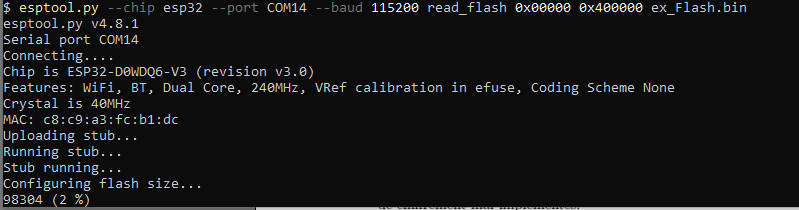
\includegraphics[scale=0.7]{./ressource/esptool}
\end{center}


\subsection{Exploitation }


\begin{minipage}{0.6\linewidth}

\begin{encadre}{Ghidra}
Ghidra est une suite d'outils d'ingénierie inverse développée par la NSA. Elle permet de désassembler et de décompiler des fichiers binaires, le dump mémoire facilitant ainsi leur analyse.
\end{encadre}
\end{minipage}
\begin{minipage}{0.35\linewidth}
\begin{center}

\includegraphics[scale=0.4]{./ressource/ghidra.png}
\end{center}
\end{minipage}

\paragraph{Installation : } Si ce n'est pas déjà effectué, lancer l'installation de Ghidra maintenant sur votre Kali. Elle peut être un peu longue.
 
Une fois qu'un fichier est importé sur Ghidra et que le processeur cible a a été configuré (ex. : \texttt{Xtensa - Little indian} pour les cartes ESP32), de multitudes d'analyse sont disponibles : 
\begin{itemize}
\itemE Utilisez l'outil \texttt{Decompiler} pour convertir le code désassemblé en une représentation pseudo-C.
\itemE Identifiez les sections de mémoire contenant des données importantes (ex. : tables de symboles, constantes)
\itemE Recherchez des chaînes de caractères pour localiser des fonctions critiques ou des paramètres systèmes
\itemE Reconstruction de code source pour comprendre les algorithmes utilisés.
\itemE Localisation de failles de sécurité, comme des fonctions vulnérables ou des mécanismes de chiffrement mal implémentés.
\itemE Extraction de secrets, tels que \textbf{des clés ou mots de passe}
\end{itemize}


\section{A vous}

\begin{enumerate}
\itemE Échanger des cartes avec vos voisins.
\itemE Récupérer les informations confidentiels que vous souhaitez. \textbf{Aides} : Vous avez à disposition une courte vidéo nommée \verb?ghidraAide.mp4? présentant \textbf{Ghidra}
\itemE Avec le script python nommée \verb?fauxClientKali.py?, se faire passer pour le capteur mais en envoyant des données erronées
\end{enumerate}

\begin{center}
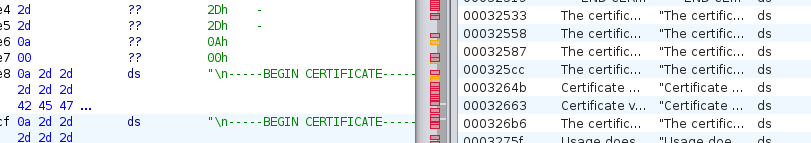
\includegraphics[scale=0.7]{./ressource/analyseMem}
\end{center}


\section{Réponse du SOC}

\begin{minipage}{0.55\linewidth}
En tant que technicien SOC, vous venez de vous apercevoir que votre système avait encore une faille. Comment y remédier :  
\end{minipage}
\begin{minipage}{0.44\linewidth}
\begin{center}

\includegraphics[scale=0.7]{./ressource/cyberHro.png}
\end{center}
\end{minipage}

\begin{itemize}
\itemE Sécuriser l'accès au capteur.
\itemE Utiliser des solutions de l'esp32 $\Rightarrow$ C'est la solution que vous, en tant que technicien du SOC, vous allez étudier
\end{itemize}


\huge
\begin{center}
\vspace{0.5cm}
\textbf{Les manipulations suivantes peuvent Hard-bricker l'esp32 
$\Rightarrow$ Je vous demande de ne pas la réaliser}
\end{center}
\vspace{0.5cm}
\normalsize

\begin{encadre}{Hard-bricked}
Etat dans lequel un dispositif électronique, comme un ESP32, est totalement inutilisable en raison de dommages irréversibles au niveau matériel ou logiciel. Cela signifie que le périphérique ne peut plus être démarré, contrôlé ou reprogrammé, même en utilisant des outils avancés de récupération.
\end{encadre}


\paragraph{Différentes solutions de sécurité} sont intégré à l'ESP32. pour y avoir accès, les plus simple est de suivire les étapes ci-dessous :

\begin{enumerate}
\item Dans un répertoire dédié, importé un projet \verb?hello_world?
\end{enumerate}

\begin{lstlisting}[style=commande]
cp -r $IDF_PATH/examples/get-started/hello_world/* .
\end{lstlisting}



\begin{enumerate}[resume]
\item Choisir la cible esp32
\end{enumerate}

\begin{lstlisting}[style=commande]
idf.py set-target esp32
\end{lstlisting}


\begin{enumerate}[resume]
\item Lancer le menu de configuration
\end{enumerate}

\begin{lstlisting}[style=commande]
idf.py menuconfig
\end{lstlisting}


\begin{enumerate}[resume]
\item Etudier les différents éléments
\end{enumerate}

\begin{center}
\includegraphics[scale=0.7]{./ressource/menuconfig}
\end{center}

\begin{enumerate}[resume]
\item Se renseigner sur les 3 éléments de sécurité \textbf{NE PAS LES METTRE EN PLACE}
\end{enumerate}


\section{Critère d'évaluation}
\label{lblCritere}
Vous serez évalué sur les points suivants :

\begin{itemize}
\itemE La description accompagné de copie d'écran de la démarche pour récupérer les informations et se faire passer pour le capteur
	\begin{itemize}
	\item[$\Rightarrow$] 3 pt : 1 pt pour chaque étape
	\end{itemize}
\itemE Présentation de la démonstration
	\begin{itemize}
	\item[$\Rightarrow$] 1 pt : fonctionnement
	\item[$\Rightarrow$] 2 pt : échange et réponse aux questions
	\end{itemize}
\itemE Une description des différentes éléments de sécurité existant et la raison de sa non-mise en place
	\begin{itemize}
	\item[$\Rightarrow$] 3pt 
	\end{itemize}

\end{itemize}

\ifPROF
\color{red}
\begin{itemize}
\itemE Require signed app images : Permet d'exécuter uniquement les images d'application signées avec une clé privée approuvée, empêchant les firmwares non autorisés. La signature est vérifiée au démarrage à l'aide d'une clé publique incluse dans le chargeur d'amorçage.

\itemE Enable hardware secure biit in booloader : Vérifie l'intégrité du chargeur d'amorçage lors de chaque démarrage grâce à une clé unique stockée dans les e-fuses. Garantit que le chargeur d'amorçage n'a pas été modifié, protégeant contre les attaques de remplacement.
\itemE Enable flash encryption on boot : Chiffre automatiquement le contenu de la mémoire flash pour empêcher l'accès non autorisé aux données sensibles. La clé de chiffrement est unique et stockée de manière sécurisée dans le matériel de l'ESP32.
\end{itemize}

\normalcolor
\fi

\end{document}
